\documentclass[12pt,a4paper]{article}
\usepackage{pdfpages}
\usepackage{ngerman}
\usepackage{algorithmic}
\usepackage{fancyhdr}
\usepackage{graphicx}

\renewcommand{\sectionmark}[1]{\markboth{\thesection\ #1}{}}
\lhead[ \leftmark   ]{\textbf{ATM}}
\rhead[]{Kai Fabian, Stefan Hansch, Dominik Moritz, Matthias Springer}
\cfoot[\thepage]{\thepage}

\begin{document}
\begin{titlepage}
\author{Kai Fabian\\Hasso-Plattner-Institut, IT-Systems Engineering, 1. Semester\\\texttt{Kai.Fabian@student.hpi.uni-potsdam.de} 
\and Stefan Hansch\\FH Regensburg, Medizinische Informatik, 1. Semester\\\texttt{Stefan.Hansch@stud.hs-regensburg.de} 
\and Dominik Moritz\\Hasso-Plattner-Institut, IT-Systems Engineering, 1. Semester\\\texttt{Dominik.Moritz@student.hpi.uni-potsdam.de}
\and Matthias Springer\\Hasso-Plattner-Institut, IT-Systems Engineering, 1. Semester\\\texttt{Matthias.Springer@student.hpi.uni-potsdam.de}}

\title{ATM\\informatiCup Aufgabe 3}

\date{\today}
\maketitle
\end{titlepage}
\pagestyle{fancy}
\tableofcontents

\section{Einf"uhrung}
Vor der Planung des eigentlichen Programmsablauf, der Entwicklung der Algorithmen und der Implementierung des Programms und der GUI haben wir uns grundlegende Gedanken zur Aufteilung des Programms gemacht und folgendes Modell entwickelt.\\
\includegraphics[width=1.0\textwidth]{scheme.pdf}
Dieses Modell entspricht nicht mehr dem aktuellem Stand, war jedoch Anfangs als ein grobes Konzept sehr hilfreich.\\
Zur Umsetzung unserer Ideen benutzten wir die NetBeans IDE unter Verwendung der Programmiersprache Java unter Windows. Unser Projekt ist sehr modular aufgebaut und in verschiedene Packages und Klassen unterteilt. Diese modulare und objektorientierte Programmentwicklung hatte insbesondere folgende Vorteile.
\begin{itemize}
\item \textbf{Teamf"ahigkeit:} Verschiedene Mitglieder eines Teams k"onnen gleichzeitig an verschiedenen Klassen/Teilen des Projekts arbeiten. Dies war besonders wichtig, weil drei Personen in Potsdam und eine Person in Regensburg am Projekt arbeitete. Als Versionsverwaltung setzten wir Subversion ein.
\item \textbf{Leichte Austauschbarkeit von Quelltext:} "Anderungen, Verbesserungen und neue Algorithmen k"onnen ohne gro"sen Aufwand implementiert werden.
\end{itemize}
Die Dokumentation wurde mit \LaTeX\ (TeX Live 2010) erstellt.
\section{Installationsanleitung}
Wie in der Dokumentation beschrieben, setzten wir die Aufgabe in Java mithilfe der NetBeans
IDE um. Mit NetBeans ist es sehr einfach m"oglich, den Code zu untersuchen und das Programm neu zu kompillieren. 

Um das Programm zu starten, ist  aber nur die Java Runtime Environment (JRE) oder eine vergleichbare Java VM erforderlich. Um das Programm zu starten, gen"ugt es, die Datei \texttt{informaticup.jar} im Ordner \texttt{Programm} auszuf"uhren. Falls das Programm so nicht gestartet werden kann (wegen einer falsch gesetzten \texttt{PATH} Variable), l"asst sich das Programm auch mit dem Befehl \texttt{java -jar ``informaticup.jar``} starten. Wichtig ist, dass der Ordner \texttt{lib} mit den Bibliotheken immer neben der Programmdatei liegt, damit die Bibliotheken geladen werden k"onnen.
\section{Bedienungsanleitung}
Wir schrieben eine benutzerfreundliche, m"oglichst selbsterkl"arende  Benutzeroberfl"ache f"ur unser Programm. Die wichtigsten Bedienelemente sind im folgendem dokumentiert.

Im Men"upunkt Berechnung gibt es zwei Unterpunkte. Der eine startet eine komplett neue Berechnung, der andere bearbeitet eine bereits bestehende Berechnung. Beide bestehen weitgehend aus denselben Komponenten.

Wir w"ahlen "`Berechnung"'  $\rightarrow$ Untermen"u   "`Neue Berechnung"' $\rightarrow$ Es "offnet sich ein neues Fenster. Mit "`Lade Datei"' kann die entsprechende Eingabedatei ausgew"ahlt werden.
Ist die Karte ausgew"ahlt, hat der Benutzer weitere Einstellungsm"oglichkeiten.
\begin{itemize} 
\item Auf der rechten Seite finden sich die einzelnen Attribute dieser Karte. Der Nutzer kann diese bei jeder neuen Berechnung ver"andern. Somit k"onnen die verschiedenen Einzelattribute, die in den Eingabedatei stehen, unterschiedlich stark gewichtet werden.
\item Mittig unter "`keine Berechnung"' kann die Karte ohne Automaten in unser Hauptfenster eingezeichnet werden. Gewichtskarte bedeutet, dass die Karte die entsprechend gew"ahlten Attribute bereits umsetzt.
\item Auf der linken Seite, kann der Algorithmus ausgew"ahlt werden, mit dem die Automaten auf dieser Karte gesetzt werden. Es gibt zwei Arten von Algorithmen: Die Er"offnungsalgorithmen sowie die Optimierungsalgorithmen. (Unterschiede siehe Algorithmendokumentation)
Bei den Optimierungsalgorithmen, kann die Suchintensit"at eingestellt werden. Ab einer gen"ugend hohen Suchintensit"at, empfiehlt es sich, den Er"offnungsalgorithmus "`Zufall"' zu w"ahlen, da der vorherrgehende Algorithmus keinen signifikanten Einfluss mehr auf die G"ute der L"osung hat. Falls andere als die vorgegebenen oder von uns erzeugten Beispiele verwendet werden (insbesondere bei einer sehr gro"sen Anzahl an Automaten), kann es dennoch sinnvoll sein, den Greedy-Algorithmus zu verwenden.
\item Im unteren Teil kann die Approximationsrate noch ver"andert werden. Die Approximationsrate gibt an, wie stark die Karte verkleinert wird, damit ggf. schnellere Berechnungen erfolgen k"onnen. Zur Auswahl steht die manuelle oder automatische Auswahl der Approximationsrate. Wird sie automatisch gesetzt, so wird diese in Abh"angigkeit des Arbeitsspeichers des entsprechden PCs gew"ahlt. Durch die Auswahl per Hand kann je nach den entsprechenden Bed"urfnissen eine h"ohere oder niedrigere Approximationsrate gew"ahlt werden.
\end{itemize}
Ist die Auswahl getroffen, so wird nach erfolgreicher Eingabe wieder ins Hauptfenster gewechselt. Die angezeigte Karte kann vergr"o"sert oder verkleinert werden. Vielmehr k"onnen die Automaten auch g"anzlich entfernt werden oder zus"atzliche Automaten "uber den Men"upunkt "`Automaten"' gesetzt werden. Will man nicht alle Automaten automatisch setzen lassen, so m"ussen diese entsprechend markiert werden. W"ahlt man nun "`Berechnung"' bearbeiten, so k"onnen die Standpunkte der restlichen Automaten (wie bereits zuvor erw"ahnt) optimiert werden.
Jeder Zustand (wie die Automaten stehen und welches Gewicht sie haben) kann unter dem entsprechenden Men"upunkt gespeichert werden.

\subsection{Eine Beispielberechnung}
Programm Starten  $\rightarrow$ "`Berechnung"' $\rightarrow$ "`Neue Berechnung"' $\rightarrow$ "`Lade Datei"'. Hier w"ahlen wir Hatfield.txt aus. Wir belassen die Attribute alle auf 1, lassen die Approximationsrate automatisch setzen und w"ahlen "`Zeige Pixelkarte und berechne Gewichtskarte"' aus.

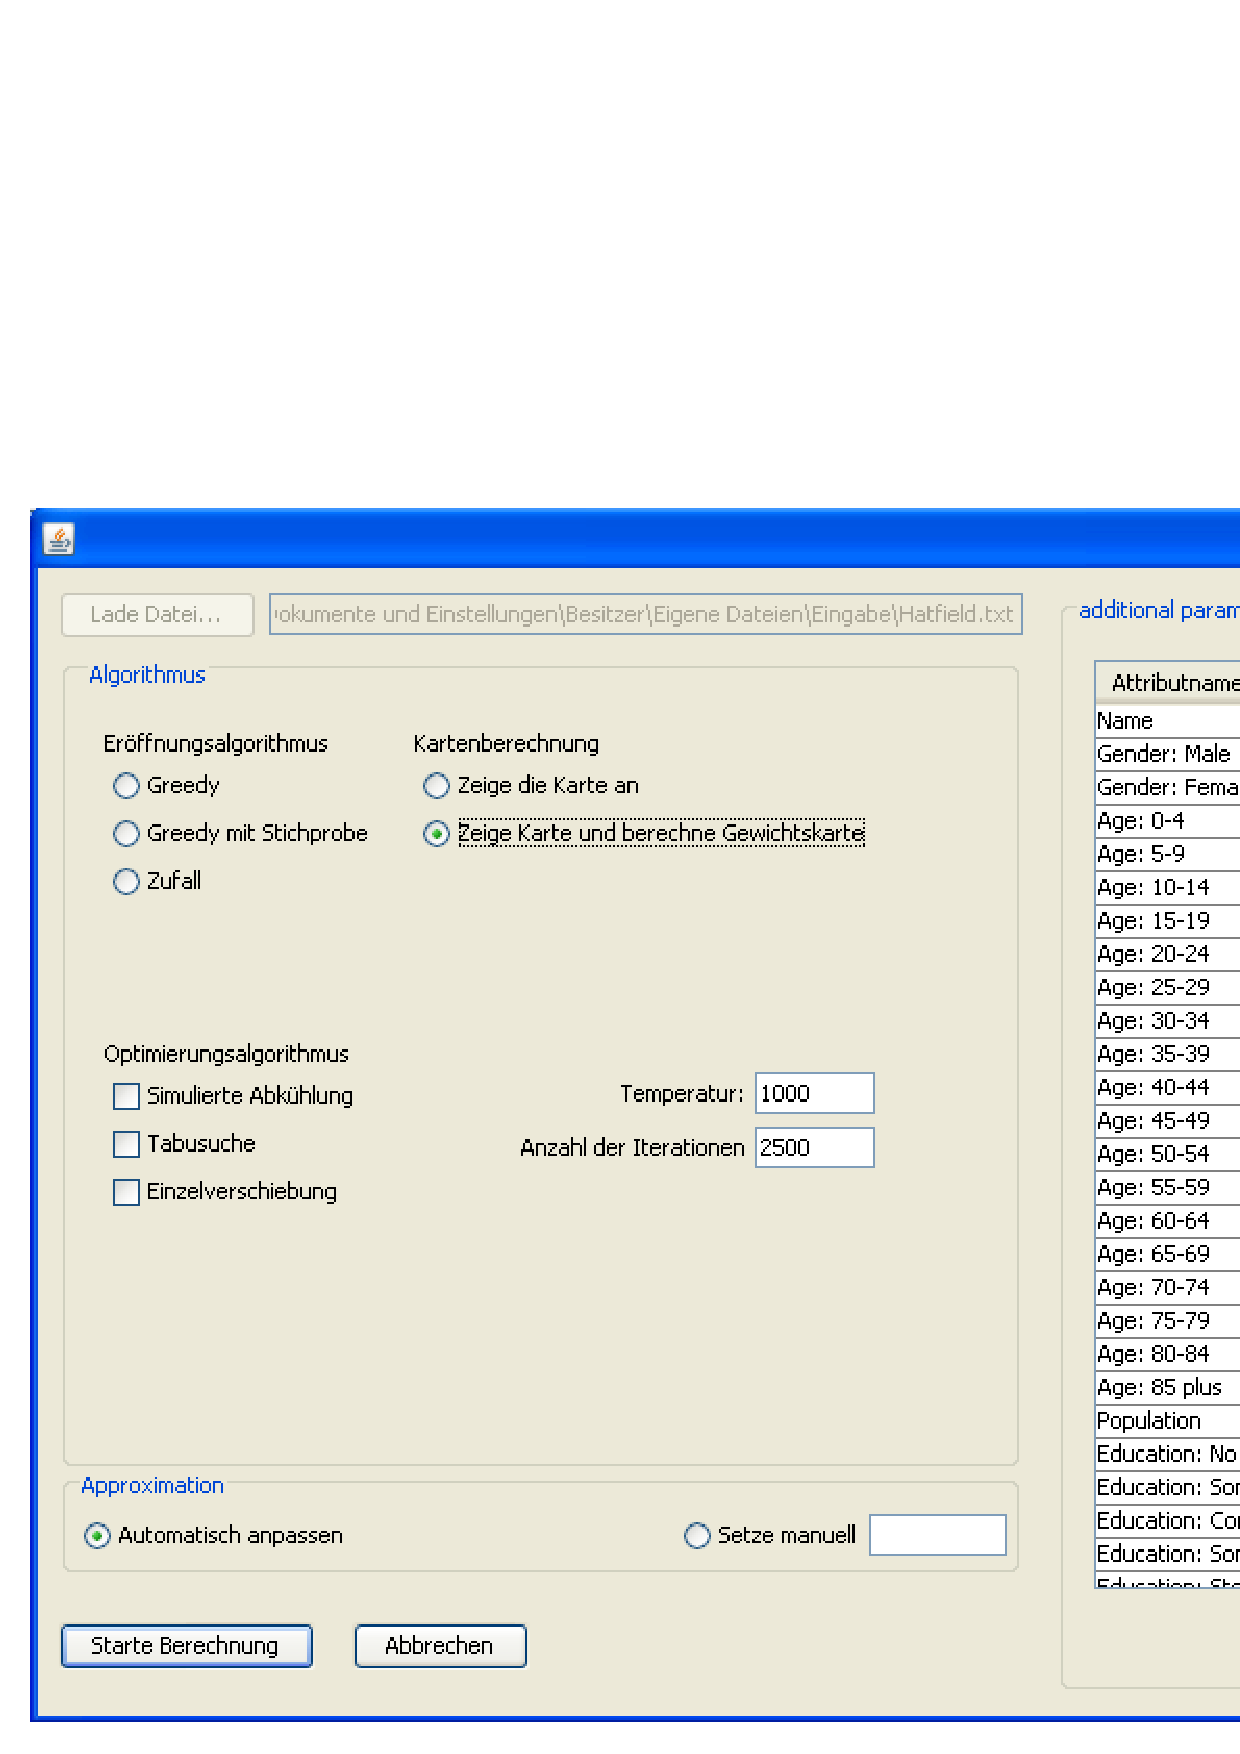
\includegraphics[width=0.5\textwidth]{Gewichtskarte.pdf}

Durch Klicken auf "`Starte Berechnung"' erscheint in etwa folgende Karte.

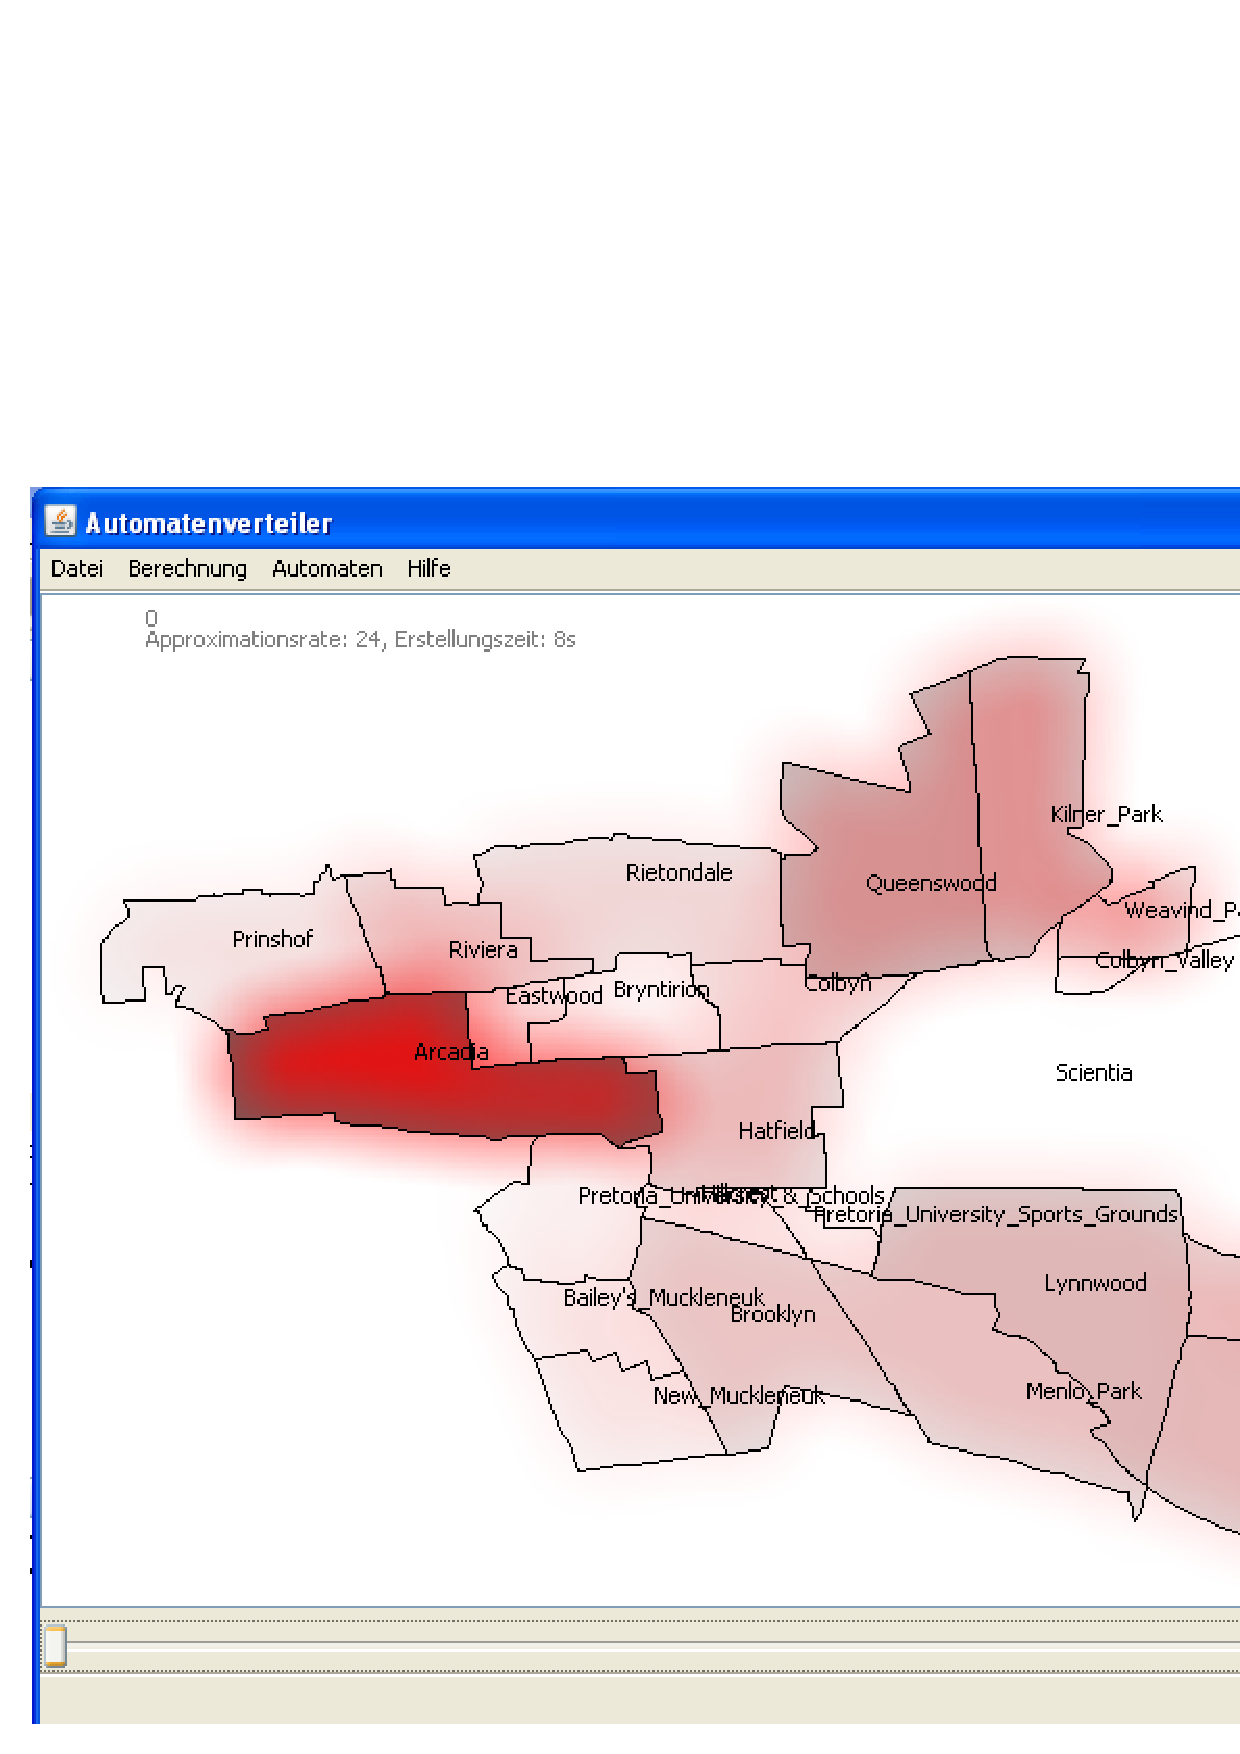
\includegraphics[width=0.5\textwidth]{Gewichtskarte2.pdf}

Nun setzen wir "uber "`Automaten"' $\rightarrow$ "`Neuer Automat"' einen neuen Automaten. Dieser ist fest verankert, kann aber durch entsprechende Men"uauswahl entsperrt werden. Wir f"uhren nun "`Berechnung"'  $\rightarrow$ "`Berechnung bearbeiten "' aus. Hier w"ahlen wir den Greedy-Algorithmus aus und zus"atzlich alle Optimierungsalgorithmen.

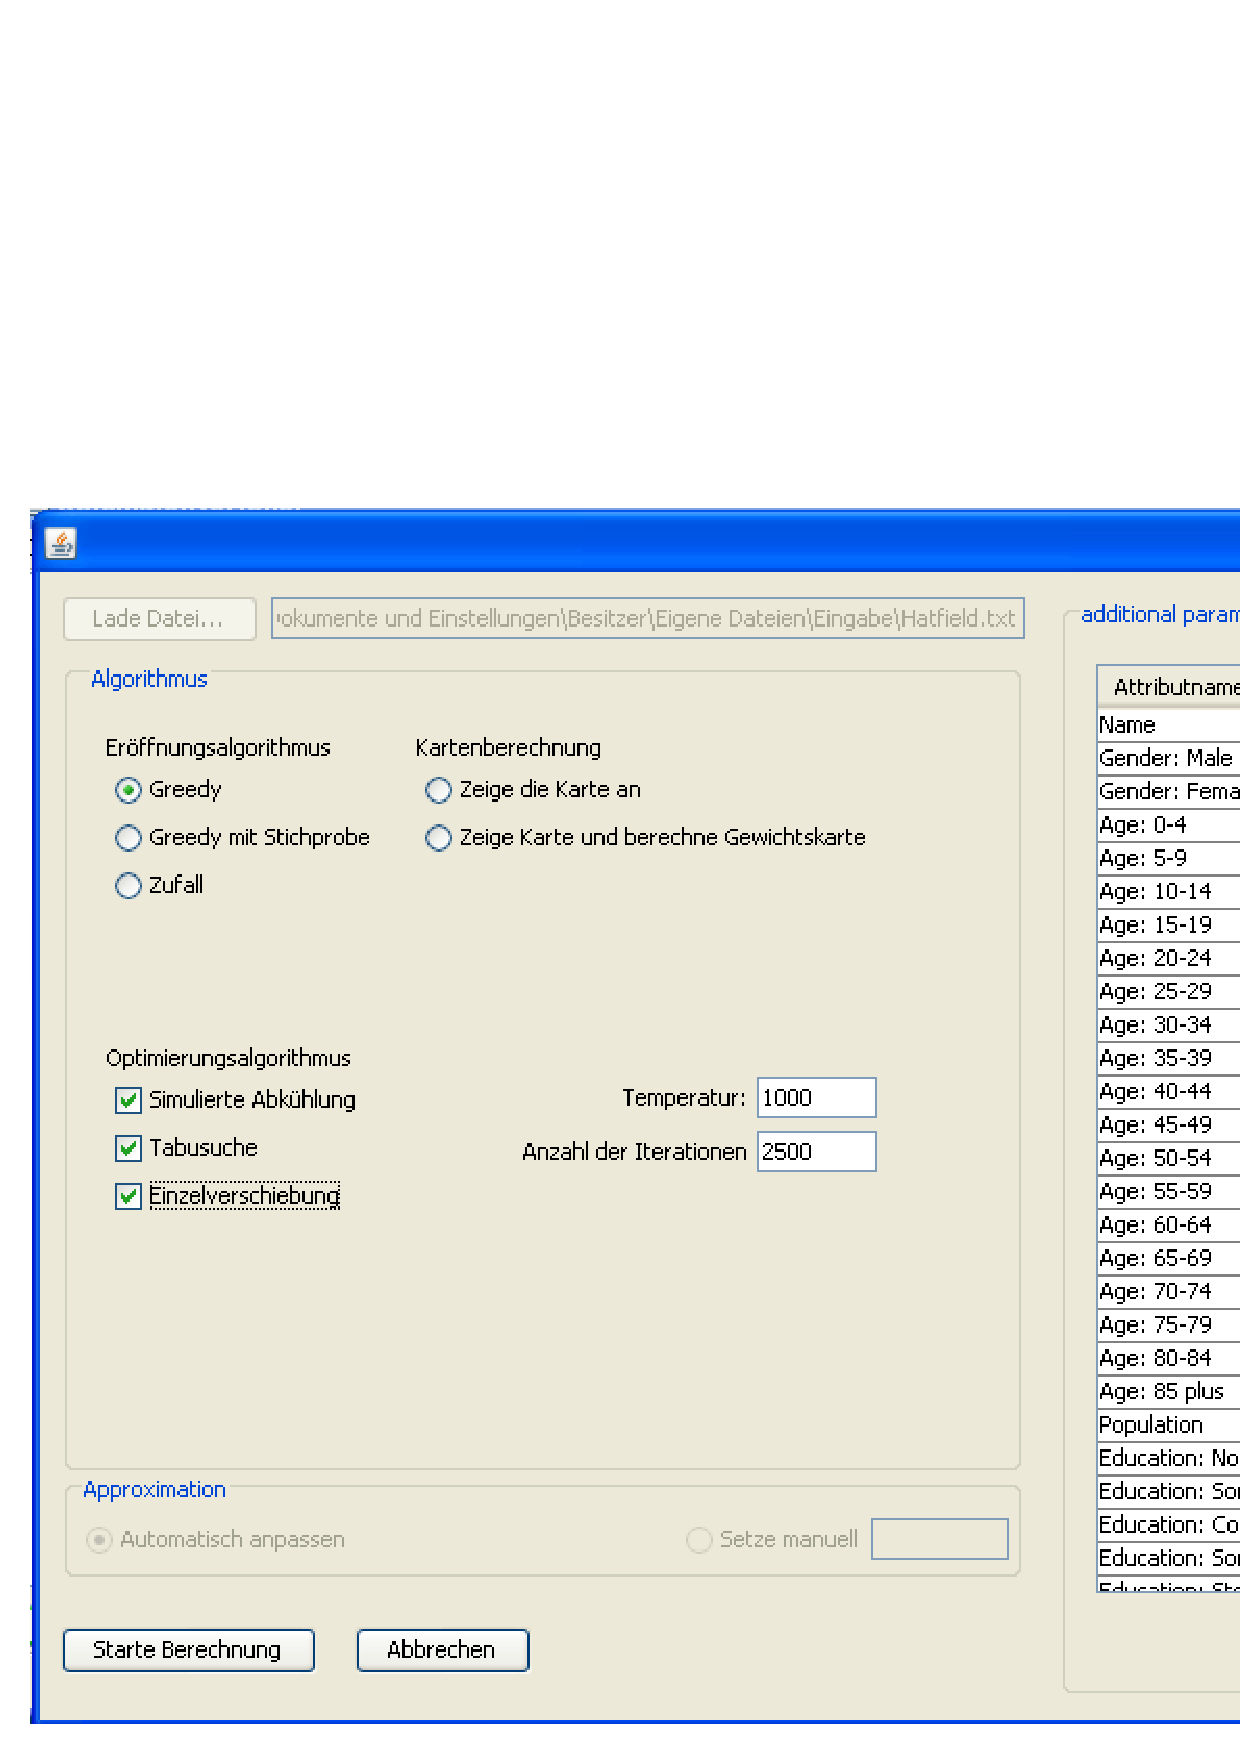
\includegraphics[width=0.5\textwidth] {Allealgos2.pdf}

Sieht dann folgenderma"sen aus.

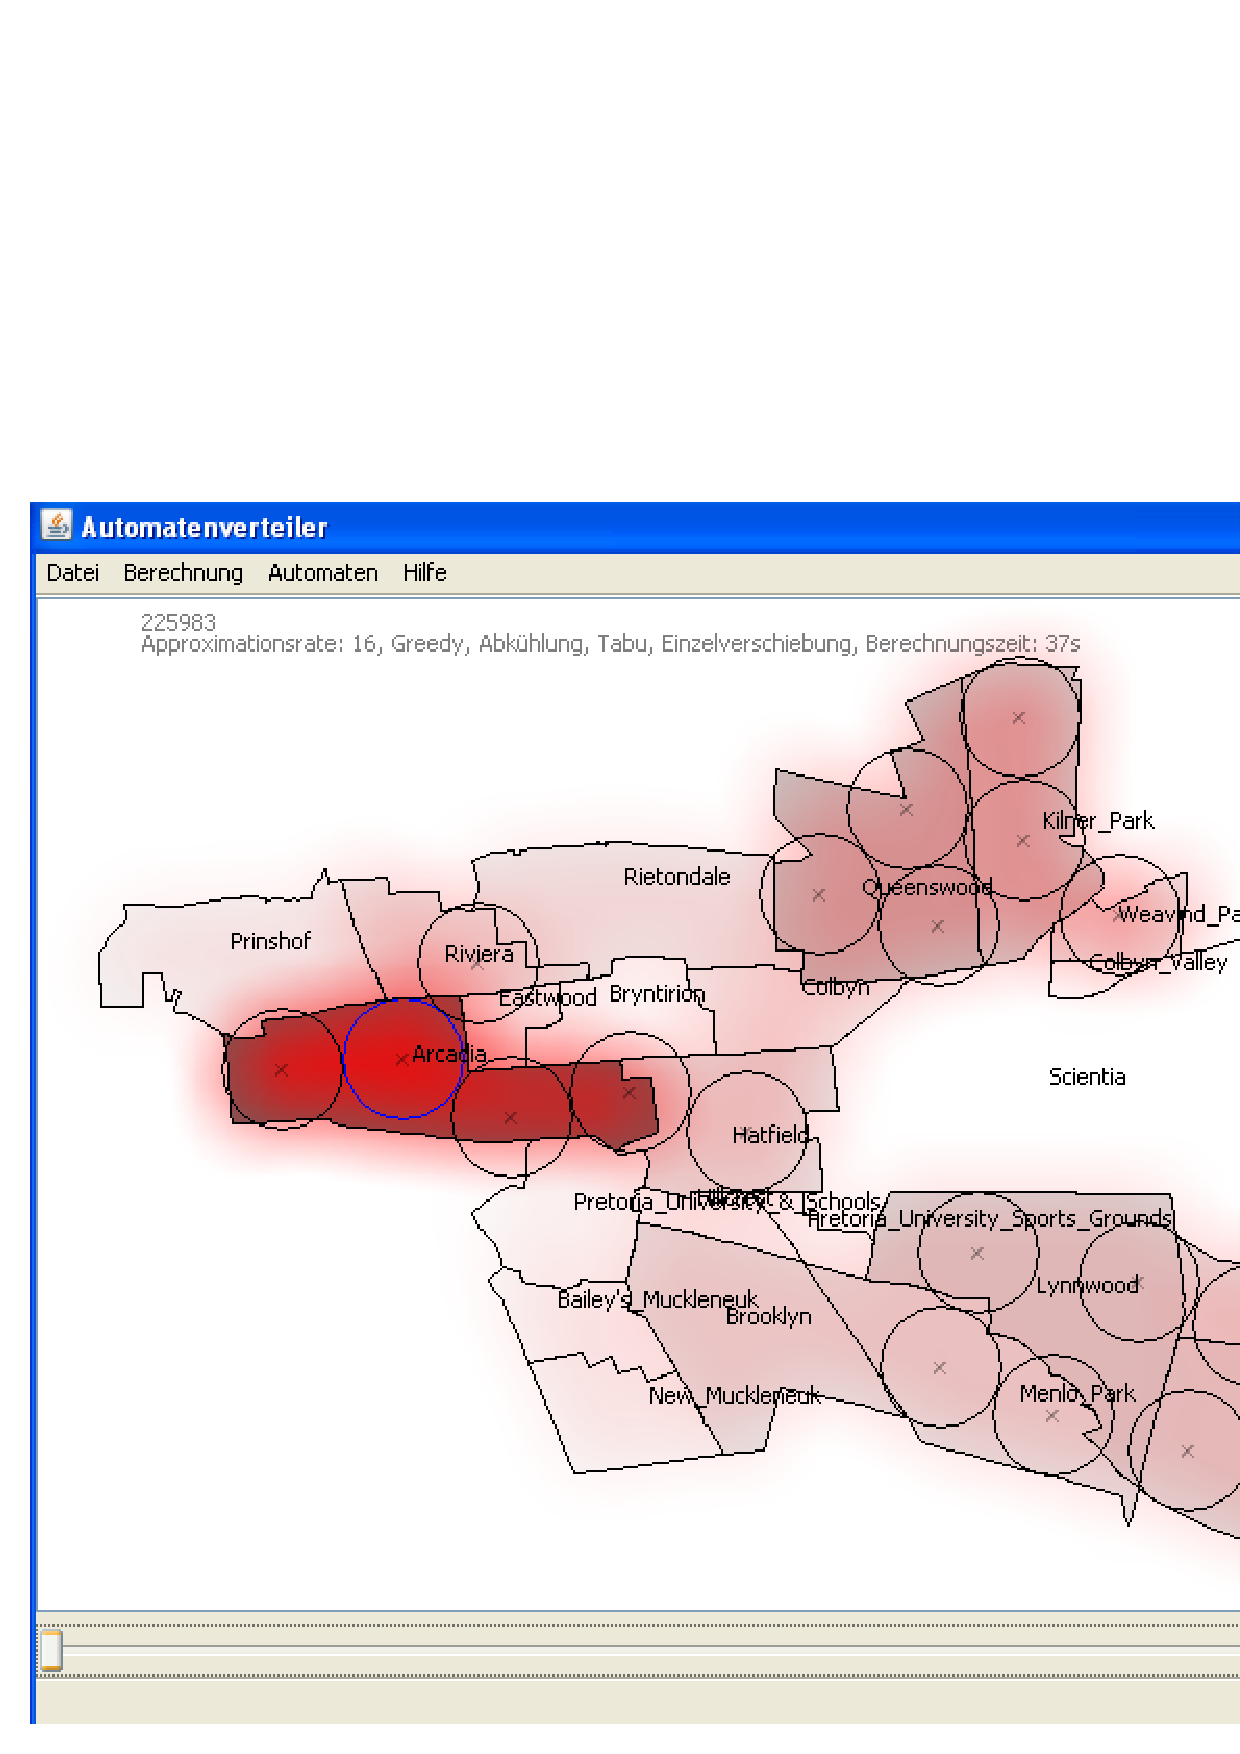
\includegraphics[width=0.5\textwidth] {AlleAlgos.pdf}

Zuletzt speichern wir das Ganze mit "`Datei"' $\rightarrow$ "`Speichern"'.
\section{Datenstruktur}
\subsection{Grunds"atzliches in aller K"urze}
\begin{itemize}
\item \textbf{Approximationsrate:} Um schneller an Ergebnisse zu kommen, werden Karten verkleinert und somit sind weniger Daten zu verarbeiten.
\item \textbf{Automat, Stadtteil, Koordinate:} Klassen, in welchen die wichtigsten Daten der einzelnen Automaten, Stadtteile, Koordinaten gespeichert sind.
\item \textbf{Karte:} Karte, die aus einzelnen Pixeln besteht, und f"ur jeden Pixel einen Wert enth"alt.
\item \textbf{Welt:} Speichert die wichtigsten Parameter, wie die einzelnen Stadtteile, die Pixelkarte, den Radius der Automaten oder die Anzahl der Automaten, jedoch keine L"osung des Problems. Die Positionen der einzelnen Automaten werden hier also \emph{nicht} gespeichert.
\item \textbf{Zustand:} Ausgehend von einer Welt wird hier gespeichert, wo die Automaten stehen und welches Gewicht sie haben.
\end{itemize}

\subsection{Automat}
Wie der Name schon sagt beschreibt die Klasse \texttt{in"-fo"-ma"-ti"-cup."-da"-ten"-struk"-tur."-Au"-to"-mat} einen Automaten. Es werden keine Berechnungen durchgef"uhrt, sondern nur Informationen "uber einen einzelnen Automaten gespeichert. Dazu geh"oren Position und Radius des Automaten, sowie ein Wahrheitswert, der angibt, ob der Automat gesperrt ist. Wenn ein Automat gesperrt ist, darf er nicht gel"oscht werden und seine Position darf nicht ver"andert werden.

\subsection{Koordinate}
Die Klasse \texttt{in"-for"-ma"-ti"-cup."-da"-ten"-struk"-tur."-Ko"-or"-di"-na"-te} wird f"ur die Speicherung der Positionen der Automaten sowie der Punkte der Polygone der Stadtteile verwendet. Die Klasse enth"alt keine Algorithmen oder Berechnungsschritte. 

\subsection{Pixelkarte}
\paragraph{L"osungsidee}
Die Pixelkarte ist eine Konvertierung der Welt als Vektorkarte in eine Pixeldarstellung. Sie enth"alt einzelne Stadtteile, deren Begrenzungen keine Vektoren mehr sind, sondern Striche auf einer Pixelkarte. 

Bei der Erzeugung der Pixelkarte wird die Karte automatisch skaliert (approximiert). Wird beispielsweise ein Approximationsfaktor von \(2\) angegeben, so werden s"amlichte vorkommende Koordinaten durch \(2\) geteilt. Die Aufl"osung der Karte wird also effektiv durch den Faktor \(4\) geteilt. Der Approximationsfaktor kann entweder manuell eingegeben werden oder automatisch ermittelt werden. Dadurch kann das Programm auch extreme Eingabedateien mit einer gro"sen Kartenbreite oder -h"ohe verarbeiten. Gro"se Eingabedateien werden einfach heruntergerechnet auf kleinere Eingabedateien. Nat"urlich nimmt dadurch auch die Aufl"osung und damit die Genauigkeit der L"osung ab. Die Geschwindigkeit der Algorithmen nimmt daf"ur zu. Wie genau der Zusammenhang zwischen der Geschwindigkeit der Algorithmen und der Gr"o"se der Karte aussieht, kann den Laufzeitabsch"atzungen der einzelnen Algorithmen entnommen werden.

Die Pixelkarte speichert f"ur die einzelnen Pixel keine Farben, sondern Gewichte. Ein Pixel kann sich in einem bestimmten Stadtteil befinden, dem nach der Gewichtungsfunktion der Attribute ein bestimmter Gewichtswert zugewiesen wurde. Jeder Pixel in einem Stadtteil erh"alt das Gewicht des betreffenden Stadtteils geteilt durch die Anzahl an Pixel im Stadtteil als Wert. Summiert man nun beispielsweise nur die H"alfte der Pixel des Stadtteils auf, erh"alt man nur die halbe Bewertung des Stadtteils.

\paragraph{Programm-Dokumentation}
Die Koordinaten der einzelnen Stadtteile wurden zuvor vom Parser erstellt, dabei wurden einfach die Werte aus der Eingabedatei "ubernommen. Die Methode \texttt{in"-for"-ma"-ti"-cup."-Welt"-funk"-ti"-on."-Approxi"-ma"-ti"-on} skaliert (approximiert) die Karte um einen bestimmten Approximationsfaktor. Dazu werden einfach alle Koordinaten der Polygone aller Stadtteile durch den Approximationsfaktor geteilt. Ebenso wird der Radius der Automaten durch den Approximationsfaktor geteilt. 

Nun beginnt die eigentliche Berechnung der Pixelkarte. Dazu werden Java-interne Funktionen verwendet, da diese einseits sehr schnell und andererseits bei extremen Eingabedaten (z.B. Stadtteilen, die aus keinem Pixel bestehen) nicht anf"allig f"ur Fehler sind\footnote{Diesen Teil hatten wir urspr"unglich komplett selbst geschrieben.}. Die Funktion \texttt{in"-for"-ma"-ti"-cup."-Welt"-funk"-ti"-on."-er"-stelle"-Pix"-el"-kar"-te} erstellt die eigentliche Pixelkarte. Dazu werden die Stadtteile als gef"ullte Polygone auf ein \texttt{Buffered"-Image} geschrieben. Danach werden die einzelnen Pixel aus dem Bild ausgelesen und in ein Array geschrieben, auf das effizienter zugegriffen werden kann. Anf"angliche Probleme gab es, weil das Gewicht durch die Anzahl der Pixel geteilt wird und dadurch Werte enstanden, die kleiner als 1 sind. Das \texttt{Buffered"-Image} unterst"utzt jedoch nur Ganzzahlen. Als L"osung wird ein zweites \texttt{Buffered"-Image} erstellt, das angibt, durch welchen Wert jeder Pixel geteilt werden soll.

\paragraph{Laufzeitabsch"atzung}
Das Skalieren (Approximieren) der Karte h"angt lediglich linear von der Anzahl der Koordinaten ab, die verarbeitet werden sollen. Wie schnell das Zeichnen der Polygone geht, ist uns nicht genau bekannt, da diese Aufgabe von Java-Bibliotheken "ubernommen wird. Das "Ubertragen der einzelnen Pixel-Werte in das Array h"angt linear von der Anzahl der Pixel und damit der Gr"o"se der Karte ab. Die Skalierung beschleunigt diesen Prozess nur um einen konstanten Faktor. 
\subsection{Stadtteil}
Die Klasse \texttt{in"-for"-ma"-ti"-cup."-da"-ten"-struk"-tur."-Stadt"-teil} wird f"ur die Speicherung der Stadtteile verwendet. F"ur jeden Stadtteil werden die Name und Werte der einzelnen Attribute gespeichert, sowie die Eckpunkt der Polygone, die den Stadtteil abgrenzen, wobei diese Punkte Koordinaten auf der Pixelkarte sind. Das Gewicht eines Stadtteils, das aus der Gewichtung der Attribute ergibt, wird in der Variable \texttt{\_ge"-wicht"-Nach"-Fkt} gespeichert.

Der einzige Berechnungsschritt in dieser Klasse ist die Berechnung der Fl"ache des Polygons (Methode \texttt{be"-rech"-ne"-Ne"-ben"-effek"-te}). Diese ergibt sich nach der gau"sschen Trapezformel.
\begin{equation}2 A=\sum_{i=1}^n (y_i + y_{i+1})(x_i-x_{i+1})\end{equation}
Die Laufzeit dieses Berechnungsschrittes h"angt linear von der Anzahl der Punkte eines Polygons ab.


\subsection{Welt}
Die Klasse \texttt{in"-for"-ma"-ti"-cup."-da"-ten"-struk"-tur."-Welt} beschreibt die Probleminstanz ohne den Zustand, also ohne die L"osung (Automaten). Die Welt besteht aus den einzelnen Stadtteilen, dem Radius der Automaten, der Anzahl der zu platzierenden Automaten und der Pixelkarte. Die L"osung des Problem wird sp"ater in einen \texttt{Zu"-stand} geschrieben. In der \texttt{Welt} wird au"serdem der Approximationsfaktor gespeichert. Die \texttt{Welt} wird jedoch nur approximiert, wenn die entsprechende Methode in der \texttt{Welt"-funk"-ti"-on} aufgerufen wird.

\subsection{Gewichtskarte}

\paragraph{L"osungsidee}
Da viele Algorithmen simulieren, wie Automaten an den verschiedensten Stellen bewertet w"urden, war eine "Uberlegung um die Programmeffizienz zu steigern, eine zweidimensionale Karte vorauszuberechnen, die f"ur jede Koordinate die erwartete Bewertung beinhaltet. Da der Radius eines Automaten durch die Eingabedatei festgelegt ist, kann diese von fast jedem Algorithmus ben"otigte Gewichtskarte vorausberechnet werden.
Urspr"unglich wurde f"ur jede Koordinate \texttt{(x, y)} das umliegende Quadrat mit der Kantenl"ange des Kreisdurchmessers \texttt{[(x-r..x+r),(y-r..y+r)]} betrachtet: Mittels des Satzes des Pythagoras wurde bestimmt, ob der Punkt innerhalb des umliegenden Kreises liegt, und falls dies zutrifft, das Gewicht des darunter befindlichen Stadtteiles \texttt{getGewicht(x, y)} zu einer spezifischen Summe der Koordinate hinzuaddiert.
Dieses Verfahren war "au"serst ineffizient, da f"ur jede m"ogliche Koordinate viele Berechnungen durchgef"uhrt werden mussten.
Um dies zu vermeiden, wurde die folgende Optimierung vorgenommen: In einer separaten Variable der Gr"o"se \texttt{short Kreis = [2r, 2r]} wurde ein derartiger Kreis mittels pythagor"aischer Betrachtung vorberechnet. Sofern der Punkt im Kreis lag (also die Bedingung $(x-r)^2+(y-r)^2 \leq r^2$ erf"ullt ist) enth"alt das Kreisarray an der Stelle \texttt{(x,y)} den Wert \texttt{1}, ansonsten \texttt{0}. Aufsummiert wurde nun nicht mehr \texttt{getGewicht(x, y)}, sondern \texttt{getGewicht(x, y) * Kreis[x][y]}.
Um die ben"otigte Zeit zur Berechnung der Gewichtskarte weiter zu reduzieren, wurden die so genannten \textbf{Deltakreise} eingef"uhrt. Es ist n"amlich zu erkennen, dass das Gewicht des Pixels \texttt{(x+1, y)} auch aus dem Gewicht des Punktes \texttt{(x, y)} berechnet werden kann. Selbiges gilt f"ur \texttt{(x, y+1)} und \texttt{(x, y)}. Deshalb werden vergleichbare Arrays (\texttt{short deltakreis\_rechts = [2r+1, 2r]} und \texttt{short deltakreis\_unten = [2r, 2r+1]}) vorausberechnet, um die Anzahl der notwendigen Operationen weiter zu reduzieren. Dem Bildbereich dieser beiden Arrays wurde der Wert \texttt{-1} hinzugef"ugt. Als Berechnungsanweisung wird der gleiche Algorithmus wie f"ur den normalen Kreis angewandt (\textit{Multiplikation des Gewichts mit dem Inhalt des Arrays}).

% \paragraph{Programm-Dokumentation}

\paragraph{Laufzeitabsch"atzung}
Das Generieren der Gewichtskarte h�ngt von mehreren Faktoren ab: Von der Kartengr"o"se \texttt{Welt"-funk"-ti"-on."-get"-Max"-i"-ma"-le"-Brei"-te"-Hoehe(true) = A}, den Automatenradien \texttt{Welt.getRadiusAutomaten() = r} und dem Approximationsfaktor \texttt{Welt.getApproxrate() = a}. F"ur jeden Punkt der approximierten Karte, also insgesamt $ \frac{A}{a} $ Punkte, m"ussen die Referenz-/Deltakreis-Arrays durchlaufen werden, welche widerum eine Gr"o"se von $ 4 * r^2 $, bzw. vernachl"assigbar $ 4 * r * (r+1) $ besitzen. Daraus folgt, dass je Koordinate $ \frac{A * 4 * r^2}{a} $ Vergleichsoperationen durchgef"uhrt werden m"ussen. Das Ergebnis der Vergleichsoperation bestimmt, ob ein Wert addiert (subtrahiert) werden muss. Durchschnittlich findet dies alle $ \frac{2*2}{\pi} = \frac{4}{\pi} $ Koordinaten statt.

\subsection{Zustand}
Die Klasse \texttt{in"-for"-ma"-ti"-cup."-da"-ten"-struk"-tur."-Zu"-stand} beschreibt die L"osung einer Probleminstanz, also wo die einzelnen Automaten platziert worden sind. Dazu gibt es ein Array \texttt{\_au"-to"-ma"-ten}. Im Zustand werden au"serdem die Bewertung der aktuellen L"osung und ein Zeiger auf die Gewichtskarte gespeichert. Die Gewichtskarte ist nur "uber den Zustand erreichbar und wird beim ersten Zugriff erstellt und gespeichert. Erfolgen sp"ater weitere Zugriffe auf die Gewichtskarte, muss diese nicht neu berechnet werden. In dieser Klasse befinden sich deshalb auch der Algorithmus zur Berechnung der Gewichtskarte. 

Vor der Berechnung der Automatenpositionen durch die Algorithmen wird bereits ein Automaten-Array mit der korrekten Gr"o"se erstellt, welches jedoch nur \texttt{null}-Zeiger enth"alt. Somit kann bereits vor Ausf"uhrung eines Algorithmus durch die GUI auf das Automaten-Array zugegriffen werden, um einzelne Automaten per Hand zu erstellen. 


\section{Typischer Programmablauf}
Ein typischer Programmablauf mit Anwendung der Algorithmen und Generieren einer Ausgabedatei sieht wie folgt aus.
\begin{enumerate}
\item Benutzer l"adt eine Eingabedatei durch Ausw"ahlen einer Datei im Dateiauswahl-Dialog.
\begin{enumerate}
\item Parser liest die Eingabedatei ein und erzeugt eine \texttt{Welt} (\texttt{in"-for"-ma"-ti"-cup."-create"-Calc"-Frame."-start"-Parsing}).
\item Attribute werden aus der \texttt{Welt} ausgelesen und in die Tabelle hinzugef"ugt (\texttt{in"-for"-ma"-ti"-cup."-create"-Calc"-Frame."-load"-File})
\end{enumerate}
\item Benutzer gewichtet die Attribute in der Tabelle (optional).
\item Benutzer startet den Berechnungvorgang (\texttt{in"-for"-ma"-ti"-cup."-In"-for"-ma"-ti"-cup"-View."-start"-Cal"-cu"-lation}).
\begin{enumerate}
\item Gewichtung der einzelnen Attribute wird ausgewertet und die Stadtteile erhalten ihr Gewicht \texttt{\_ge"-wicht"-Nach"-Fkt} (\texttt{in"-for"-ma"-ti"-cup."-create"-Calc"-Frame."-be"-rei"-te"-Be"-rech"-nung"-Vor}).
\item Parameter und ausgew"ahlte Algorithmen werden ausgewertet, Variablen werden gesetzt (\texttt{in"-for"-ma"-ti"-cup."-In"-for"-ma"-ti"-cup"-View."-start"-Cal"-cu"-lation}), neuer Task f"ur die Berechnung wird erstellt (\texttt{in"-for"-ma"-ti"-cup."-In"-for"-ma"-ti"-cup"-View."-Start"-Cal"-cu"-lation"-Task."-do"-In"-Back"-ground}).
\item Koordinaten werden approximiert/skaliert (\texttt{in"-for"-ma"-ti"-cup."-Welt"-funk"-ti"-on."-Approx"-i"-ma"-ti"-on}).
\item Wenn kein Algorithmus ausgew"ahlt wurde und die Karte nur gezeichnet werden soll: Neuer \texttt{Zu"-stand} wird erstellt, das hei"st, bereits gesetzte Automaten werden verworfen.
\item Pixelkarte wird erstellt (\texttt{in"-for"-ma"-ti"-cup."-Welt"-funk"-ti"-on."-er"-stelle"-Pix"-el"-kar"-te}).
\item Wenn bisher noch kein \texttt{Zu"-stand} existiert: Erstelle neuen \texttt{Zu"-stand}. Bestehende Automaten werden nicht gel"oscht.
\item Gewichtskarte wird erzeugt (\texttt{in"-for"-ma"-ti"-cup."-da"-ten"-struk"-tur."-Zu"-stand."-er"-zeu"-ge"-Ge"-wichts"-kar"-te}).
\item F"uhre Er"offnungsalgorithmus aus (Greedy, Greedy mit Strichproben, Zufall oder Backtracking).
\item F"uhre Optimierungsalgorithmus aus (Simulierte Abk"uhlung, Tabu-Suche, und/oder Einzelverschiebung).
\item Zeichne die L"osung (Klasse \texttt{in"-for"-ma"-ti"-cup."-draw"-ing"-Panel}).
\end{enumerate}
\item Benutzer speichert die L"osung (\texttt{in"-for"-ma"-ti"-cup."-Da"-tei"-ex"-port."-da"-tei"-Aus"-ge"-ben}).
\end{enumerate}

\subsection{Dateieingabe und Dateiausgabe}
Eine Datei wird sofort geladen, wenn der Benutzer die Datei im Dateiauswahl-Dialog "offnet. Die Klasse \texttt{in"-for"-ma"-ti"-cup."-Da"-tei"-im"-port} ist daf"ur zust"andig, die komplette Datei erst einmal in eine Zeichenfolge zu lesen. Diese kann dann vom Parser \texttt{in"-for"-ma"-ti"-cup."-Par"-ser} zu einer \texttt{Welt} verarbeitet werden. Dabei werden die einzelnen Stadtteile erzeugt, die Attribute ausgelesen und Radius und Anzahl der Automaten ermittelt. Schl"agt dieser Vorgang fehl, wird eine \texttt{Par"-ser"-Ex"-ception} geworfen.

Wenn alle Berechnung abgeschlossen sind, liegt ein \texttt{Zu"-stand} vor, der vom Benutzer auch nachtr"aglich noch ver"andert werden kann. Er kann beispielsweise Automaten verschieben. Ein solcher \texttt{Zu"-stand} kann durch die Methoden in der Klasse \texttt{in"-for"-ma"-ti"-cup."-Da"-tei"-ex"-port} dann in eine Ausgabedatei geschrieben werden, die die in der Aufgabenstellung geforderte Form hat. 

\subsection{Weltfunktion}
Die Klasse \texttt{in"-for"-ma"-ti"-cup."-Welt"-funk"-ti"-on} enth"alt Operationen und Funktionen, die auf die \texttt{Welt} angewandt werden k"onnen. Dabei handelt es sich um das Erstellen der Pixelkarte (siehe Kapitel \emph{Zustand}) und das Approximieren der Koordinaten. 

Au"serdem existiert eine Funktion, die die maximale Breite bzw. H"ohe der Karte ermittelt. Dieser Wert ist notwendig, um automatisch einen guten Wert f"ur die Approximation zu finden. Die Karte wird dann so approximiert, dass bei jeder Karte etwa gleich gro"se Pixelkarten entstehen, die in vern"unftiger Zeit verarbeitet werden k"onnen. Gro"se Karten werden also st"arker verkleinert als kleine Karten. 


\section{Algorithmen}
\subsection{Modularer Aufbau}
Aufgrund einer Vielzahl von m"oglichen Algorithmen, haben wir uns dazu entschlossen, eine vom Algorithmus unabh"angige Datenstruktur und Benutzeroberfl"ache zu entwerfen. Diese Datenstruktur erm"oglicht es, viele Algorithmen zu testen und somit den \emph{besten} Algorithmus zu finden. Hinzu kommt, dass durch viele Algorithmen auch Spezialf"alle leichter betrachtet werden k"onnen.

\subsection{G"ute einer L"osung}
Bei dem gegebenen Problem, Automaten m"oglichst effizient auf einer Landkarte zu verteilen, handelt es sich um ein Optimierungsproblem. Damit eine L"osung als g"ultig (zul"assig) klassifiziert wird, m"ussen die folgenden Kriterien erf"ullt sein.
\begin{itemize}
\item Es m"ussen alle Automaten auf der Landkarte platziert sein.
\item Jeder Automat muss auf der Landkarte und darf nicht au"serhalb der Karte platziert sein.
\item Die Bereiche (Kreise) der Automaten d"urfen sich nicht "uberschneiden.
\end{itemize}
F"ur g"ultige L"osungen kann dann die \emph{G"ute} berechnet werden. Je h"oher dieser Wert ist, desto besser ist die L"osung (Maximierungsproblem). Jedem Pixel wurde zuvor bereits ein Gewicht zugewiesen. Die G"ute einer L"osung ergibt sich aus der Summe der Gewichte aller Pixel, an denen sich ein Automat befindet. Da die einzelnen Pixel in der Pixelkarte bereits Gewichtswerte enthalten, die durch die Anzahl der Pixel im Stadtteil geteilt wurden, ergibt sich eine anteilsm"a"sige der G"ute an den Stadtteilen. Wenn ein Stadtteil von einem Automaten nur zu 40 Prozent abgedeckt wird, gibt es f"ur diesen Automaten nur 40 Prozent der Bewertung des Stadtteiles.

\subsection{Brute-Force-Suche}
Eine erste Idee war ein Brute-Force-Algorithmus. Das w"urde in unserem Programm bedeuten, dass jeder einzelne Punkt der Karte auf seinen Automatenwert untersucht wird. Ein solcher Algorithmus w"urde zu einer optimalen L"osung f"uhren. Allerdings ist dieser Algorithmus nicht performant genug. 

Wenn man annimmt, dass die Landkarte aus \(p\) Pixel besteht, so gibt es f"ur jeden Automaten \(p\) M"oglichkeiten, ihn zu platzieren. Nat"urlich d"urfen sich die Automatenradius nicht "uberschneiden, sodass sich etwas weniger m"ogliche Positionen ergeben. Da die abgedeckte Fl"ache eines Automaten aber in der Regel viel kleiner als die Landkarte ist, kann man diesen Effekt bei der Laufzeitbetrachtung vernachl"assigen. Sollen \(a\) Automaten platziert werden, ergeben sich \(\mathcal{O}(p^a)\) m"ogliche Zust"ande (exponentielle Laufzeit), die "uberpr"uft werden m"ussen. Mit einem Zustand eine m"ogliche Platzierung aller \(a\) Automaten gemeint.  Bereits bei \(a=2\) Automaten k"onnen die vorgegebenen Beispieleingaben nicht mehr in sinnvoller Zeit berechnet werden. 

\subsection{Zuf"allige Verteilung der Automaten}
Vor allem als Er"offnungsverfahren f"ur Metaheuristiken kann es interessant sein, eine zuf"allige g"ultige L"osung zu erzeugen. Dabei werden einfach alle Automaten per Zufall auf der Karte verteilt, wobei sich Automaten nicht "uberschneiden d"urfen. Der Algorithmus befindet sich in der Klasse \texttt{al"-go"-rith"-men."-Zu"-fall} und die Laufzeit h"angt quadratisch von der Anzahl der Automaten ab, da f"ur jeden Automaten "uberpr"uft werden muss, ob er sich mit irgendeinem anderen Automaten "uberschneidet. 

\subsection{Heuristiken}
Heuristiken bezeichnen in der Informatik solche Vorgehensweisen, bei denen ein Kompromiss zwischen dem Rechenaufwand und der G"ute der gefundenen L"osung eingangen wird. Mit sehr gro"ser Wahrscheinlichkeit findet die Heuristik also nicht die/eine optimale L"osung, daf"ur wird versucht, eine gute Ann"aherung in akzeptabler Zeit zu ermitteln. 

\subsubsection{Greedy-Algorithmus mit vollst"andiger Suche}
\paragraph{Grundprinzip}
Der Greedy-Algorithmus (engl. \emph{greedy} = gierig) w"ahlt zu jedem Zeitpunkt den Schritt, der momentan am meisten Erfolg verspricht. Dieses Verfahren f"uhrt in der Regel nicht dazu, dass eine optimale L"osung gefunden wird. Ebenso kann nicht garantiert werden, dass die gefundene L"osung eine bestimmte Mindestg"ute aufweist, die gefundene L"osung kann beliebig schlecht sein. Andererseits funktioniert das Verfahren relativ schnell. 

\paragraph{Pseudocode}
Der Algorithmus geht bei der Berechnung nach folgendem Prinzip vor.

\begin{algorithmic}
\FOR{$i = 1$ \TO Automaten}
	\STATE Beste Position $\gets -1$
	\FOR{$x = 1$ \TO $max_x$}
		\FOR{$y = 1$ \TO $max_y$}
			\IF{Bewertung(x, y) $>$ Beste Position}
				\STATE Beste Position $\gets$ Bewertung(x, y)
				\STATE best$_x$ $\gets x$
				\STATE best$_y$ $\gets y$
			\ENDIF
		\ENDFOR
	\ENDFOR
	\STATE Setzte Automat(best$_x$, best$_y$)
\ENDFOR
\RETURN best$_x$, best$_y$
\end{algorithmic}
Der erste Schritt besteht darin, den Pixel mit dem maximalen Gewicht zu finden. Hat man diesen gefunden, platziert man an dieser Stelle den ersten Automaten. Dieser Schritt wird nun so lange wiederholt, bis alle Automaten platziert wurden. Es muss jedoch darauf geachtet werden, dass sich die Automatenkreise nicht "uberschneiden. Bevor ein Automat platziert wird, muss deshalb sichergestellt sein, dass der Abstand zu jedem anderen Automaten mindestens den doppelten Automatenradius betr"agt\footnote{Diese "Uberpr"ufung auf G"ultigkeit fehlt der "Ubersicht halber im Pseudocode.}. Im allgemeinen kann der erste Pixel der Landkarte, anders als im Pseudocode angegeben, auch eine andere Koordinate als \((1|1)\) aufweisen. 

\paragraph{Laufzeitkomplexit"at}
Besteht die Landkarte aus \(p = \mbox{max}_x \cdot \mbox{max}_y\) Pixeln, so m"ussen f"ur jeden Automaten \(p\) Pixel untersucht werden. F"ur jeden interessanten Pixel muss nun noch der Abstand zu allen anderen Pixel "uberpr"uft werden. Sollen \(a\) Automaten platziert werden, sind \(\theta(a \cdot p)\) Vergleiche der Pixelgewichte und \(\mathcal{O}(a^2 \cdot p)\) Abstandsberechnungen notwendig. Normalerweise ist \(a\) im Gegensatz zu \(p\) sehr klein und kann vernachl"assigt werden.

\paragraph{Programm-Dokumentation}
Der Greedy-Algorithmus befindet sich in der Klasse \texttt{al"-go"-rith"-men."-Greedy} und implementiert das Interface \texttt{in"-for"-ma"-ti"-cup."-Al"-go"-rith"-mus}. Der eigentliche Algorithmus startet, wenn die Methode \texttt{Be"-rech"-ne} aufgerufen wird. Die Methode \texttt{Setze"-Naechsten"-Au"-to"-ma"-ten} platziert den n"achsten Automaten und verwendet dazu die Methode \texttt{Fin"-de"-Bes"-te"-Po"-si"-ti"-on"-Voll"-staen"-dige"-Suche}, die "uber alle Pixel iteriert. Die Funktion \texttt{Punkt"-Zu"-laess"-ig} ermittelt, ob an der angegebenen Position ein Automat platziert werden darf, indem der Abstand zu allen bereits gesetzten Automaten berechnet wird.

\subsubsection{Greedy-Algorithmus mit Stichproben-Suche}
\paragraph{Grundprinzip}
Der vorgestellte Algorithmus kann beschleunigt werden, wenn nicht alle Pixel auf ihr Gewicht "uberpr"uft werden. Stattdessen wird die Karte horizontal oder vertikal in zwei gleich gro"se Teile (Kartenausschnitte) aufgeteilt. Dann wird aus beiden Teilen eine Stichprobe von \(s\) Pixeln entnommen. F"ur jeden Teil werden die Gewichte der ausgew"ahlten Pixel aufsummiert. Dann wird der Teil mit der gr"o"seren Summe erneut aufgeteilt. Eine horizontale Teilung erfolgt, wenn der betrachtete Kartenausschnitt eine gr"o"sere Breite als H"ohe aufweist. Ansonsten wird vertikal geteilt. Wenn ein Kartenausschnitt aus nur noch einem Pixel besteht, endet das Verfahren. Unter allen insgesamt ausgew"ahlten Pixeln wird der Pixel mit dem maximalen Gewicht als neuer Automatenstandort festgelegt. Nat"urlich muss noch sichergestellt werden, dass kein Pixel ausgew"ahlt wird, sodass sich die Automatenkreise "uberschneiden. 

Dieses Verfahren ist vor allem dann sinnvoll, wenn man annimmt, dass sich Stadtteile mit einer guten Gewichtung nebeneinander befinden. Der Algorithmus betrachtet die Karte zun"achst sehr grob. Die Stellen, die besonders gut aussehen, betrachtet er dann n"aher. Au"serdem kann man davon ausgehen, dass Stadtteile relativ gro"s sind und viele Pixel umfassen. In allen Pixeln eines Stadtteils ist das Gewicht gleich. Deshalb kann man bereits bei einer relativ kleinen Anzahl an Stichproben mit gro"ser Sicherheit einen guten Pixel finden.

\paragraph{Pseudocode}
Der Algorithmus geht bei der Berechnung nach folgendem Prinzip vor.

\begin{algorithmic}
\STATE Punkt 1 $\gets (1|1)$
\STATE Punkt 2 $\gets (\mbox{max}_x|\mbox{max}_y)$
\STATE Bester Punkt $\gets -1$
\WHILE{Bereich gro"s genug}
	\STATE Teil A/B Punkt 1/2 $\gets$ Teile Bereich()
	\STATE Stichproben$_{A/B} \gets 0$
	\FOR{$i = 1$ \TO Stichprobengr"o"se}
		\STATE Punkt$_A \gets$ Stichprobe(Teil A Punkt 1, Teil A Punkt 2)
		\STATE Punkt$_B \gets$ Stichprobe(Teil B Punkt 1, Teil B Punkt 2)
		\STATE Stichproben$_A \gets$ Stichproben$_A$ + Bewertung(Punkt$_A$)
		\STATE Stichproben$_B \gets$ Stichproben$_B$ + Bewertung(Punkt$_B$)
		\STATE Bester Punkt $\gets \max$ (Punkt$_A$, Punkt$_B$, Bester Punkt)
	\ENDFOR
	
	\IF{Stichproben$_A >$ Stichproben$_B$}
		\STATE Punkt 1 $\gets$ Teil A Punkt 1
		\STATE Punkt 2 $\gets$ Teil A Punkt 2
	\ELSE
		\STATE Punkt 1 $\gets$ Teil B Punkt 1
		\STATE Punkt 2 $\gets$ Teil B Punkt 2
	\ENDIF
\ENDWHILE
\RETURN Bester Punkt
\end{algorithmic}
Im Pseudocode fehlt die "Uberpr"ufung der Punkte auf G"ultigkeit der "Ubersichtlichkeit halber. Ein Bereich, aus dem Stichproben entnommen werden k"onnen, ist durch zwei Punkte definiert, dem Punkt links oben (Punkt 1) und dem Punkte rechts unten (Punkt 2). Anders als Pseudocode muss die Karte nicht notwendigerweise mit dem Pixel \((1|1)\) beginnen\footnote{Analog zum Greedy-Algorithmus mit vollst"andiger Suche}. Stichproben werden zuf"allig aus dem angegebenen Bereich entnommen.

\paragraph{Laufzeitkomplexit"at}
Es ist sinnvoll, die Gr"o"se der Stichprobe an die Gr"o"se der Karte zu koppeln, da bei gr"o"seren Karten auch gr"o"sere Stichproben ben"otigt werden. Die Gr"o"se der Stichprobe ergibt sich aus \(s = q \cdot r\), wobei \(r\) die Gr"o"se des Kartenausschnitts (Anzahl der Pixel) und \(q\) das Verh"altnis der zu entnehmenden Pixel bezogen auf den Kartenausschnitt ist. Im ersten Schritt wird die Karte in zwei gleich gro"se Teile geteilt und es werden zweimal (f"ur jeden Kartenausschnitt) \(0,5 \cdot p \cdot q\) Pixel ausgew"ahlt (\(p\) ist die Gr"o"se der Karte). Im n"achsten Durchlauf werden zweimal \(0,25 \cdot p \cdot q\) Pixel ausgew"ahlt. Pro Automat werden also \(\sum_{i=0}^{\infty} 2^{-i} \cdot p \cdot q = 2 \cdot p \cdot q\) Pixel untersucht. Somit untersucht der Algorithmus insgesamt \(\theta(a \cdot 2 \cdot p \cdot q)\) Pixel. In der Implementation des Algorithmus wurde \(q = 0,1\) gesetzt. 

\textbf{Hinweis:} In der Regel ist bereits der Greedy-Algorithmus schnell genug. Beide Greedy-Algorithmen waren bei unseren Tests (vorgegebene Testf"alle) so schnell, dass sich kein wirklicher Unterschied feststellen l"asst. 

\paragraph{Programm-Dokumentation}
Der Greedy-Algorithmus mit Stichproben-Suche befindet sich ebenfalls in der Klasse \texttt{al"-go"-rith"-men."-Greedy}. Falls der Parameter \texttt{\_stich"-pro"-ben} auf \texttt{true} gesetzt ist, wird der Stichproben-Algorithmus statt der vollst"andigen Suche verwendet. Die Funktion \texttt{Fin"-de"-Bes"-te"-Po"-si"-ti"-on"-Stich"-pro"-ben"-Su"-che} ermittelt die neue Position, an der ein Automat platziert werden soll. Die Abbruchbedingung der \texttt{while}-Schleife ist die "Uberpr"ufung, ob der betrachtete Bereich nur noch aus wenigen Pixeln besteht. Jede entnommene Stichprobe wird automatisch daraufhin untersucht, ob der Pixel besser als alle zuvor untersuchten Pixel ist. Der insgesamt beste entnommene Pixel (Stichprobe) wird als Ergebnis der Funktion zur"uckgegeben. Dadurch, dass der Algorithmus gute Bereiche n"aher untersucht, werden aus diesen guten Bereichen mehr Stichproben entnommen, als aus anderen Bereichen. Es gibt eine Klasse \texttt{Greedy"-Stich"-pro"-be}, die keinen Algorithmus-Quelltext enth"alt, sondern nur die \texttt{Greedy}-Klasse mit den entsprechenden Parametern aufruft. 

\subsubsection{Optimierung durch Verschiebung einzelner Automaten}
\paragraph{Grundprinzip}
Dieser Algorithmus f"uhrt eine Abschlussoptimierung einer bestehenden L"osung durch. Es muss also bereits eine L"osung vorliegen. Es wird dann jeder Automat einzeln untersucht und "uberp"uft, ob sich in der unmittelbaren Nachbarschaft des Automaten eine bessere Position befindet. Eine Position ist genau dann besser, wenn sich durch die "Anderung die G"ute der L"osung verbessert.

\paragraph{Pseudocode}
Der Algorithmus geht bei der Berechnung nach folgendem Prinzip vor.

\begin{algorithmic}
\STATE $L \gets$ Bestehende L"osung()
\STATE $G \gets$ G"ute(L)
\FOR{$i = 1$ \TO 3}
	\STATE $A \gets$ Mischen(Automaten)
	\FORALL{$a \in A$}
		\FORALL{$n \in$ Nachbarschaft(a)}
			\IF{G"ute(n) $> G$}
				\STATE $L \gets n$
				\STATE $G \gets$ G"ute(n)
			\ENDIF
		\ENDFOR
	\ENDFOR
\ENDFOR
\RETURN L
\end{algorithmic}
Bevor der Algorithmus beginnen kann, ben"otigt er eine bestehende zul"assige L"osung, die zum Beispiel vom Greedy-Algorithmus oder einer Metaheuristik (n"achstes Kapitel) erstellt wurde. Als Vergleichswert wird die G"ute dieser L"osung berechnet. 

Nun folgen drei Durchl"aufe. In jedem Durchlauf werden alle Automaten in zuf"alliger Reihenfolge sequentiell bearbeitet. F"ur jeden Automaten wird die Nachbarschaft generiert, die alle L"osungen enth"alt, bei denen der ausgew"ahlte Automat um bis zu eine Radienbreite in jede Richtung verschoben sein kann. Falls in der Nachbarschaft eine bessere L"osung existiert, wird diese ausgew"ahlt und "ubernommen. Nat"urlich werden nur zul"assige L"osungen akzeptiert, bei denen sich die Automaten nicht "uberschneiden\footnote{Auf die "Uberpr"ufung auf Zul"assigkeit wurde, wie auch bei allen anderen Pseudocodes, der "Ubersichtlichkeit halber im Pseudocode verzichtet.}.

\paragraph{Laufzeitkomplexit"at}
Die Laufzeit dieses Algorithmus h"angt linear von der Anzahl der Automaten und der Gr"o"se der Nachbarschaft ab. Die "Uberpr"ufung, ob ein Automat an einer zul"assigen Position gesetzt wurde, geht in linearer Zeit (in Abh"angigkeit von \(a\)), da in jedem Schritt nur ein einziger Automat verschoben wird. Wenn der Radius der Automaten \(r\) betr"agt und \(a\) Automaten vorliegen, hat der Algorithmus eine Laufzeit von \(\mathcal{O}(a^2 \cdot 4r^2)\).

\paragraph{Programm-Dokumentation}
Der Algorithmus befindet sich in der Klasse \texttt{al"-go"-rith"-men."-Ein"-zel"-ver"-schieb"-ung} und implementiert das Interface \texttt{in"-for"-ma"-ti"-cup."-Al"-go"-rith"-mus}. Der eigentliche Algorithmus befindet sich in der Methode \texttt{Be"-rech"-ne}. Um in einem Durchlauf einen zuf"alligen Automaten auszuw"ahlen, wird ein Array \texttt{au"-to"-mat} mit den Indizes der Automaten erstellt. Dieses Array wird von der Funktion \texttt{Mi"-sche"-Array} zuf"allig durcheinandergemischt, indem jedes Element mit einem zuf"alligen Element vertauscht wird. Die genaue Bedeutung der einzelnen Variablen und Funktionen kann dem gut dokumentierten Quelltext entnommen werden. 

\subsection{Metaheuristiken}
Im Gegensatz zu Heuristiken sind Metaheuristiken nicht auf ein spezifisches Problem beschr"ankt. Sie beschreiben allgemeine Vorgehensweisen zur L"osung von Problemen einer bestimmter Art. Wir haben zwei verschiedene Metaheuristiken - Simulierte Abk"uhlung und Tabu-Suche - implementiert, die beide in etwa nach folgendem Prinzip vorgehen.
\begin{enumerate}
\item Ermittle eine Initiall"osung mit einem beliebigem Er"offnungsverfahren.
\item Durchsuche die (lokale) Nachbarschaft der aktuellen L"osung.
\item W"ahle die beste gefundene L"osung aus der Nachbarschaft aus.
\end{enumerate}
Ein Er"offnungverfahren ist ein erster Algorithmus, der eine zul"assige Anfangsl"osung findet. Je besser diese Anfangsl"osung ist, desto einfacher kann die Metaheuristik sp"ater gute L"osungen finden. Als Er"offnungsverfahren k"onnen beispielweise alle Automaten zuf"allig verteilt werden, sofern diese zuf"allige Verteilung zul"assig ist. Besser ist jedoch, die Initiall"osung mit dem Greedy-Algorithmus zu generieren. 

Die Nachbarschaft einer zul"assigen L"osung ist die Menge von L"osungen, die aus der aktuellen L"osung durch elementare Operationen erzeugt werden k"onnen. Eine elementare Operation k"onnte zum Beispiel das Verschieben eines Automaten um wenige Einheiten sein. 

\subsubsection{Anwendbarkeit von Metaheuristiken}
Metaheuristiken k"onnen bei unserem Problem angewandt werden, weil es sich um ein kombinatorisches Optimierungsproblem handelt, d.h. die Menge der (g"ultigen) L"osungen ist diskret und aufz"ahlbar. Durch elementare Operationen, wie z.B. das Verschieben eines Automaten, kann jede L"osung, also auch eine optimale L"osung, erreicht werden.

Laufzeitprobleme k"onnen sich dann ergeben, wenn die lokale Nachbarschaft einer L"osung zu gro"s ist, um alle Nachbarn zu "uberpr"ufen. Deshalb betrachten die implementierten Metaheuristiken immer nur eine zuf"allig ausgew"ahlte Teilmenge der Nachbarschaft. 

Die G"ute der durch die Metaheurisitik gefundenen L"osung kann nicht abgesch"atzt werden. Die gefundene L"osung kann beliebig schlecht sein. W"ahlt man die Parameter (z.B. Temperatur bei Simulierter Abk"uhlung) der Algorithmen g"unstig, so erh"alt man in der Regel sehr gute Ergebnisse.

\subsubsection{Simulierte Abk"uhlung (simulated annealing)}
\paragraph{Grundprinzip}
Simulierte Abk"uhlung ist die Nachbildung des physikalisches Prozesses der Abk"uhlung eines Metalles. Anfangs hat das Metall eine sehr hohe Temperatur und die Atome im Metall befinden sich in einem sehr hohen energetischen Zustand. Durch langsame Abk"uhlung k"onnen sich die Atome so neu anordnen, dass ein energiearmer Zustand erreicht wird. K"uhlt man das Metall zu schnell ab, kann es \emph{br"uchig} werden und ist von schlechter Qualit"at. Das Metall befindet sich dann nur in einem lokal minimalen Energiezustand.

Genauso wie das Metall in einen engergie"armeren Zustand "uberf"uhrt wird, soll nun die Initiall"osung in einen energie"armeren Zustand "uberf"uhrt werden. Ein Zustand ist genau dann besonders energiearm, wenn er eine hohe G"ute aufweist. 

\paragraph{Pseudocode}
Der Algorithmus geht bei der Berechnung nach folgendem Prinzip vor.

\begin{algorithmic}
\STATE $L \gets$ Er"offnungsverfahren()
\STATE $E \gets$ Energie(L)
\STATE $T \gets$ Initialtemperatur()
\newline
\WHILE{$T > 0$}
	\FOR{$i = 1$ \TO Durchl"aufe}
		\STATE $L_{alt} \gets L$
		\FOR{$j = 1$ \TO Operationen}
			\STATE $L \gets$ ElementareOperation(L)
		\ENDFOR
		\newline
		\STATE $E_{neu} \gets$ Energie(L)
		\STATE $\Delta E \gets E_{neu} - E$
		\newline
		\IF{$\Delta E > 0$}
			\STATE $z \gets$ Zufallszahl(0, 1)
			\IF{$z \geq e^{\frac{-\Delta E}{T}}$}
				\STATE $L \gets L_{alt}$
			\ENDIF
		\ENDIF
	\ENDFOR
	\newline
	\STATE $T \gets T-1$
\ENDWHILE
\RETURN L
\end{algorithmic}
Zuerst wird mit einem Er"offnungsverfahren (z.B. Greedy-Algorithmus) eine g"ultig Initiall"osung erzeugt. Eine Bewertungsfunktion weist dieser L"osung dann ein Energieniveau zu. Je besser die L"osung ist, desto niedriger ist die Energie. Der Benutzer hat die M"oglichkeit, die Initialtemperatur beliebig festzulegen. Bei h"oheren Temperaturen dauert die Berechnung l"anger, jedoch wird auch das Ergebnis besser.

In jedem Durchlauf der While-Schleife wird die Temperatur nun um eine Einheit erniedrigt. Erst wenn die Temperatur auf Null ist, terminiert der Algorithmus: Das System ist \emph{gefroren}. F"ur jede Temperatur wird nun eine bestimmte Anzahl an \emph{Durchl"aufen} durchgef"uhrt. Jeder Durchlauf entspricht dem Generieren eines Nachbarn. Dazu wird eine bestimmte Anzahl an elementaren Operationen ausgef"uhrt. Je h"oher diese Anzahl an elementaren Operationen ist, desto weiter kann der Nachbar von der Ausgangsl"osung entfernt sein. Jedoch steigt dann auch die Wahrscheinlichkeit, dass unzul"assige L"osungen generiert werden, sodass effektiv weniger Durchl"aufe stattfinden. Der Einfachheit halber wird im Pseudocode davon ausgegangen, dass nur zul"assige L"osungen generiert werden k"onnen. 

Es wird nun das Energieniveau der neuen L"osung und die Abweichung gegen"uber der vorherigen L"osung berechnet. Falls dieser Delta-Wert gr"o"ser als Null ist, hat sich die L"osung verbessert und sie wird akzeptiert. Wurde die L"osung jedoch schlechter, so wird sie nur mit einer gewissen Wahrscheinlichkeit angenommen. Die Metropolis-Regel besagt, dass die schlechtere L"osung nur mit einer Wahrscheinlichkeit von \(e^{\frac{-\Delta E}{T}}\) (Akzeptierungsfunktion) akzeptiert wird. W"urde man nur bessere L"osungen akzeptieren, w"urde der Algorithmus ziemlich sicher in einem lokalen Energieminimum steckenbleiben. 

Die Akzeptierungsfunktion bildet auf einen Bereich zwischen \(0\) und \(1\) ab. Um mit der Wahrscheinlichkeit der Akzeptierungsfunktion zu akzeptieren, wird eine Zufallszahl zwischen \(0\) und \(1\) gebildet. Ist die Zufallszahl kleiner als der Wert der Akzeptiertungsfunktion wird akzeptiert. Ansonsten werden alle elementaren Operationen im aktuellen Durchlauf r"uckg"angig gemacht. Nach einigen Durchl"aufen wird die Temperatur erniedrigt. 

\paragraph{Verbesserungen und Erweiterungen}
Der Algorithmus wurde um einige Ideen erweitert, um ihn leistungsf"ahiger zu machen.
\begin{itemize}
\item \textbf{Variable Gr"o"se der elementaren Operationen.} Es ist m"oglich, die Gr"o"se der elementaren Operationen, also der Verschiebungen der Automaten, von der Temperatur abh"angig zu machen. So werden dann die Automaten bei einer hohen Temperatur st"arker verschoben als bei einer niedrigeren Temperatur, was der Anschauung gen"ugt, dass sich die Atome im Metall bei hoher Temperatur schneller bewegen. 
\item \textbf{Mehrfache Anwendung des Algorithmus.} Verschiedene Probleminstanzen erfordern ggf. verfschiedene Parameter. Deshalb wird der Algorithmus nach der ersten Ausf"uhrung bei niedrigerer Initialtemperatur nochmals mehrere Male aufgerufen. Parameter wie die Anzahl der Durchl"aufe, die Anzahl der elementaren Operationen oder die Berechnung der elementaren Operationen in Abh"angigkeit von der Temperatur werden dabei variiert.
\item \textbf{Speichern der global besten L"osung.} Unter allen Aufrufen des Algorithmus und allen tempor"ar generierten L"osungsvorschl"agen (bei jeder Temperatur) wird die beste gefundene L"osung gespeichert. Es ist jedoch sehr wahrscheinlich, dass die gefundene L"osung nach Anwendung des Algorithmus ohnehin die \emph{global} beste gefundene L"osung ist.
\end{itemize}

\paragraph{Generieren der Nachbarn}
Jeder Durchlauf entspricht dem Generieren eines Nachbarn. In jedem Durchlauf wird eine bestimmte Anzahl an elementaren Operationen ausgef"uhrt. Eine elementare Operation ist das Verschieben eines einzigen Automaten um einen zuf"alligen Wert. H"angt die Gr"o"se der elementaren Operationen nicht von der Temperatur ab, betr"agt die maximale Verschiebung in x-Richtung\footnote{y-Richtung analog} \(max_{x} = \frac{6 \cdot \mbox{Welt Breite}}{100}\). Soll die Verschiebung dagegen in Abh"angigkeit von der Temperatur erfolgen, so betr"agt die maximale Verschiebung in x-Richtung \(max_{x} = \frac{10 \cdot T \cdot \mbox{Welt Breite}}{100 \cdot {T_{initial}}}\). Die tats"achliche Verschiebung in x-Richtung ist ein zuf"alliger Wert zwischen \(-max_x\) und \(max_x\).

\paragraph{Laufzeitkomplexit"at}
Das Laufzeitverhalten des Algorithmus h"angt linear von der Initialtempertur, der Anzahl der Durchl"aufe und der Anzahl der Operationen ab. Die "Uberpr"ufung, ob ein L"osungsvorschlag zul"assig ist, geht in \(\mathcal{O}(a^2)\), da jeder Automat mit jedem anderen Automaten verglichen\footnote{Vergleich des Abstandes} werden muss. Die G"ute einer L"osung kann in \(\mathcal{O}(a)\) ermittelt werden, da dazu nur jede Automatenposition in der Gewichtskarte nachgeschlagen werden muss. Somit ergibt sich insgesamt ein Laufzeitverhalten von \(\mathcal{O}(T \cdot \mbox{Durchl"aufe} \cdot \mbox{Operationen} \cdot a^2)\).

\paragraph{Programm-Dokumentation}
Der Abk"uhlungs-Algorithmus befindet sich in der Klasse \texttt{Ab"-kuehl"-ung} und implementiert das Interface \texttt{in"-for"-ma"-ti"-cup."-Al"-go"-rith"-mus}. Wenn die Methode \texttt{Berechne} aufgerufen wird, wird das Berechnungsverfahren gestartet. Der eigentliche Algorithmus wird dann mehrere Male aufgerufen, wobei Parameter wie die Anzahl der Durchl"aufe oder die Anzahl der Ver"anderungen pro Durchlauf ver"andert werden. Wenn die Methode \texttt{Optimiere} aufgerufen wird, startet die Simulierte Abk"uhlung. Die Methode \texttt{Ele"-men"-ta"-re"-Oper"-ation"-en} wird verwendet, um einen neuen Nachbarn (ein Durchlauf) zu erzeugen. \texttt{BerechneZustandsGuete} berechnet die G"ute (nicht Energie!) des akutellen Zustandes und wurde so auch in anderen Algorithmen "ubernommen. Bei der Methode \texttt{Ak"-zep"tiere"-Aen"-der"-ung} muss beachtet werden, dass sich die Energiedifferenz zweier Zust"ande aus der invertierten Differenz der G"ute \(-(\mbox{neue G"ute} - \mbox{alte G"ute})\) ergibt, weil das Energieniveau umso niedriger ist, je h"oher die G"ute ist. Die genaue Bedeutung und Verwendung der einzelnen Variablen kann dem gut kommentierten Quelltext entnommen werden.

\subsubsection{Tabu-Suche}
\paragraph{Grundprinzip}
Tabu-Suche ist eine Metaheuristik, die in jedem Schritt die bestm"ogliche zul"assige L"osung in der Nachbarschaft sucht und akzeptiert. Ziel ist es, eine L"osung mit einer m"oglichst hohen G"ute zu finden. Um nicht in lokalen Maxima stecken zu bleiben und um nicht \emph{im Kreis} zu laufen, werden in einer Tabu-Liste die letzten bereits besuchten L"osungen gespeichert. Diese L"osung sind von nun an \emph{tabu} und d"urfen nicht mehr besucht werden. Es wird immer die beste gefundene L"osung in der Nachbarschaft akzeptiert, unabha"angig davon, ob die aktuelle L"osung dadurch besser oder schlechter wird. W"urde man keine Tabu-Liste anlegen, w"are es beispielsweise denkbar, dass die aktuelle L"osung \(X\) einen besten Nachbarn \(Y\) hat, der jedoch schlechter als \(X\) ist. Dennoch w"urde der Algorithmus nun \(Y\) w"ahlen. Im n"achsten Schritt k"onnte der beste Nachbar erneut \(X\) sein. W"urde man nun \(X\) erlauben, h"atte man einen endlosen Kreis \(X\), \(Y\), \(X\), \(Y\), \(\ldots\). 

\paragraph{Pseudocode}
Der Algorithmus geht bei der Berechnung nach folgendem Prinzip vor.

\begin{algorithmic}
\STATE $L \gets$ Er"offnungsverfahren()
\STATE $G \gets$ G"ute(L)
\STATE $T \gets$ ()
\STATE $Beste \gets L$
\newline
\FOR{$i = 1$ \TO Iterationen}
	\REPEAT
		\STATE $L_{neu} \gets$ N"achste beste L"osung()
	\UNTIL{$L_{neu} \not \in T$}
	\newline
	\STATE $Beste \gets \max(Beste, L_{neu})$
	\STATE F"uge $L_{neu}$ zu $T$ hinzu
	\STATE Entferne alte Elemente aus $T$
\ENDFOR
\RETURN Beste
\end{algorithmic}
Der erste Schritt besteht im Generieren einer g"ultigen Initiall"osung durch ein Er"offnungsverfahren. Die G"ute der L"osung wird ebenfalls ermittelt und gespeichert. Au"serdem wird eine leere Tabu-Liste angelegt und die Variable f"ur beste bisher gefundene L"osung auf die Initiall"osung gesetzt.

Es wird nun eine bestimmte Anzahl an Iterationen ausgef"uhrt, die vom Benutzer beliebig festgelegt werden kann. In jeder Iteration wird zun"achst der beste zul"assige Nachbar gesucht. Ein Nachbar ist genau dann zul"assig wenn er gem"a"s Kapitel \emph{G"ute einer L"osung} zul"assig ist und nicht auf der Tabu-Liste auftaucht. Dieser beste zul"assige Nachbar wird dann auf die Tabu-Liste gesetzt und ggf. in die Variable f"ur die beste bisher gefundene L"osung gespeichert. Es ist sinnvoll, die Gr"o"se der Tabu-Liste zu beschr"anken, um ein (konstant) besseres Laufzeitverhalten zu erhalten. Wird die Tabu-Liste zu gro"s, werden die "altesten Elemente in der Liste entfernt. 

Implementiert man den Algorithmus genau so, wie eben beschrieben, l"auft der Algorithmus relativ langsam, weil die Menge der Nachbarn sehr gro"s ist. Nachbarn sind alle diejenigen L"osungen, bei denen ein einziger Automat horizontal, vertikal oder horizontal und vertikal um maximal den Durchmesser der Automaten verschoben ist. Die Berechnung dauert besonders lange, weil viele Iterationen durchgef"uhrt werden sollen. Deshalb wurde der Algorithmus leicht abge"andert. In jeder Iteration wird ein Automat zuf"allig bestimmt. Dann werden nur diejenigen Nachbarn generiert, die Verschiebungen des ausgew"ahlten Automaten darstellen. Ein Eintrag in der Tabu-Liste enth"alt au"serdem nur die Information, welcher Automat verschoben wurde und in welche Richtung der Automat verschoben wurde. Eine Nachbar ist genau dann tabu, wenn die inverse Operation in der Tabu-Liste auftaucht. So darf man beispielsweise einen Automaten \(X\) nicht zuerst um \((5|1)\) verschieben und im sp"ater um \((-5|-1)\) verschieben, solange sich diese Operation auf der Tabu-Liste befindet. Die L"ange der Tabu-Liste wird auf ein Zehntel der Anzahl der Iterationen gesetzt. 

\paragraph{Laufzeitkomplexit"at}
Das Laufzeitverhalten des Algorithmus h"angt linear von der Anzahl der Iterationen, der L"ange der Tabu-Liste und der Gr"o"se der Nachbarschaft ab. Wenn ein Automat den Radius \(r\) aufweist, besteht die Nachbarschaft aus maximal \(4r \cdot 4r = 16 \cdot r^2\) Elementen. Um einen Nachbarn auf G"ultigkeit zu "uberpr"ufen, sind dieses Mal nur \(a\) Tests notwendig, da nur ein einziger Automat verschoben wurde. Wenn die Gr"o"se der Tabu-Liste \(\frac{1}{10} \cdot \mbox{Iterationen}\) betr"agt, ergibt sich ein Laufzeitverhalten von \(\mathcal{O}(\frac{1}{10} \mbox{Iterationen}^2 \cdot 16r^2 \cdot a)\).

\paragraph{Programm-Dokumentation}
Der Tabu-Algorithmus befindet sich in der Klasse \texttt{al"-go"-rith"-men."-tabu} und implementiert, wie auch der Abk"uhlungs-Algorithmus, das Interface \texttt{in"-for"-ma"-ti"-cup."-Al"-go"-rith"-mus}. Die Methode \texttt{Op"-ti"-mi"-ere} enth"alt den eigentlichen Algorithmus. Die Funktion \texttt{Ge"-ner"-iere"-Nach"-bar"-schafts"-L"os"-ung} wertet den aktuellen Zustand aus und generiert f"ur einen zuf"allig ausgew"ahlten Automaten die beste zul"assige L"osung in der Nachbarschaft, die nicht tabu ist. Der R"uckgabewert der Funktion ist eine Instanz der Klasse \texttt{Aen"-der"-ungs"-vor"-schlag}, die nur die "Anderung gegen"uber dem aktuellen Zustand enth"alt. Es wird also nur gespeichert, welcher Automat um wie viele Pixel verschoben wurde. Zusammen mit dem aktuellen Zustand kann daraus der neue Zustand berechnet werden. Au"serdem wird die G"ute der des neuen Zustandes mit der "Anderung gespeichert. Ist dieser Wert w"ahrend der Berchnung einmal \(-1\), so ist der "Anderungsvorschlag entweder nicht zul"assig oder tabu. Die Tabu-Liste ist eine verkettete Liste, die mit einem \texttt{List"-Iter"-ator} in linearer Zeit durchsucht werden kann. Das Entfernen des letzten Elements und das Einf"ugen eines neuen Elements am Anfang ist in konstanter Zeit m"oglich. 

\subsection{Fest positionierte Automaten}
Es besteht die M"oglichkeit, dass der Benutzer Automaten selbst platzieren kann. Diese Automaten werden bei der Anwendung von Algorithmen (ausgenommen Backtracking) nicht gel"oscht oder verschoben. Dazu gibt es in der Klasse \texttt{Au"-to"-mat} ein Feld \texttt{\_au"-to"-mat"-Ge"-sperrt}. Wenn diese Variable auf \texttt{true} steht, wird der Automat von den Algorithmen nicht beachtet. Das hei"st, vor jeder Operation auf den Automaten wird gepr"uft, ob der Automat gesperrt ist oder nicht. Falls er gesperrt ist, werden keine "Anderungen vorgenommen. Nat"urlich werden gesperrte Automaten aber zur G"ultigkeitspr"ufung herangezogen. Es kann also nicht vorkommen, dass sich irgendein Automat mit einem gesperrten Automat "uberschneidet, es sei denn, der Benutzer platziert zwei gesperrte Automaten so, dass sie sich "uberschneiden.
\section{"Ubersicht "uber die Programmoberfl"ache}
Dieses Kapitel beschreibt, wie die GUI in Java technisch umgesetzt wurde und ist bewusst kurz gehalten, da sie f"ur die meisten \emph{Leser} wohl eher von uninteressant ist. Beim Entwurf der Oberfl"ache versuchten wir, die folgenden Grunds"atze so gut wie m"oglich zu beachten.
\begin{itemize}
\item \textbf{Zweisprachigkeit:} Das Programm enth"alt eine englischsprachige sowie eine deutschsprachige "Ubersetzung der meisten GUI-Texte. Dies wurde "uber Ressourcen-Dateien (\texttt{in"-for"-ma"-ti"-cup."-res"-ources.*}) gel"ost. 
\item \textbf{Falsche Bedienung vermeiden:} So weit es m"oglich ist, werden falsche Eingaben durch den Benutzer erst gar nicht erlaubt. So kann der Benutzer beispielsweise die Berechnung erst gar nicht starten, wenn er einen ung"ultigen Wert f"ur die Temperatur eingibt. Au"serdem kann er Automaten nicht so platzieren, dass eine ung"ultiger Zustand entsteht.
\item \textbf{Trennung von GUI und Algorithmus:} Durch die Aufteilung in Packages und verschiedene Klassen ist uns das relativ gut gelungen. Lediglich die Klasse \texttt{in"-for"-ma"-ti"-cup."-In"-for"-ma"-ti"-cup"-View} enth"alt die Steuerung des Programmablaufes. Dort werden zum Beispiel Parameter f"ur die Algorithmen ausgewertet und die einzelnen Berechnungsschritte (z.B. Algorithmen) angest"osen. Dadurch konnten wir uns jedoch Arbeit sparen, weil oft auf Parameter-Werte aus der GUI zur"uckgegriffen werden muss.
\end{itemize}

\subsection{Hauptfenster}
Das Hauptfenster \texttt{in"-for"-ma"-ti"-cup."-In"-for"-ma"-ti"-cup"-View} ist die zentrale Steuerkomponente des Programms. Von dort aus k"onnen "uber das Men"u neue Berechnungen gestartet werden und die L"osung kann in eine Textdatei exportiert werden. 

Nach der Berechnung wird der Zustand der Welt mit allen Automaten und Stadtteilen auf ein \texttt{JPanel} gezeichnet. Dabei handelt es sich jedoch nicht um regul"ares Panel, sondern um eine Erweiterung zum \texttt{in"-for"-ma"-ti"-cup."-drawing"-Panel}. Dieses modifizierte Panel enth"alt Methoden zum Zeichnen von Stadtteilen, Automaten und der Gewichtskarte. Ebenso reagiert das Panel auf Mauseingaben. Mit der Maus k"onnen neue Automaten erzeugt und bestehende Automaten verschoben, gel"oscht und gesperrt werden. Bei diesen Aktionen ist es wichtig, die Mauskoordinaten in Pixelkoordinaten der Pixelkarte umzurechnen. Das Panel erm"oglicht au"serdem das Scrollen. Wenn das Fenster zu klein f"ur die Karte ist, wenn der Slider zur Ausgabeskalierung nach rechts geschoben wurde, kann an jede beliebige Position der Karte scrollen. Eine weitere wichtige Eigenschaft des Panels ist das automatische Neu-Zeichnen des Inhaltes, zum Beispiel wenn die Gr"o"se des Fensters ver"andert wurde.

"Uber die Men"uleiste des Hauptfensters kann der Benutzer au"serdem verschiedene Modi der L"osungsbearbeitung aktivieren und deaktivieren (Automaten erstellen, l"oschen und sperren). 

\subsection{Nebenfenster}
Neben dem Hauptfenster gibt es weitere Fenster, wie die About-Box mit den Namen der Autoren und Dialog mit den Parameter-Einstellungen f"ur die Berechnung (Berechnungsdialog). Der Berechnungsdialog \texttt{in"-for"-ma"-ti"-cup."-create"-Calc"-Frame} enth"alt Textfelder, Optionsbuttons und Checkboxen f"ur die Auswahl des Algorithmus und der Festlegung der Berechnungsparameter. Eine Tabelle \texttt{JTable} enth"alt die Gewichtungen der einzelnen Attribute, die der Benutzer frei w"ahlen kann. 



\section{Beispielausgaben}
\subsection{Tabu-Suche auf zuf"alliger Verteilung mit sehr vielen Automaten (\texttt{hatfield.txt}, 240 Automaten, 50000 Iterationen, Ver"anderungen durch den Algorithmus)}
\includegraphics[width=1.0\textwidth]{1.pdf}
\includegraphics[width=1.0\textwidth]{2.pdf}
\includegraphics[width=1.0\textwidth]{3.pdf}
\includegraphics[width=1.0\textwidth]{4.pdf}
\includegraphics[width=1.0\textwidth]{5.pdf}
\includegraphics[width=1.0\textwidth]{6.pdf}
\includegraphics[width=1.0\textwidth]{7.pdf}
\includegraphics[width=1.0\textwidth]{8.pdf}
\includegraphics[width=1.0\textwidth]{9.pdf}
\includegraphics[width=1.0\textwidth]{10.pdf}
\includegraphics[width=1.0\textwidth]{11.pdf}
\includegraphics[width=1.0\textwidth]{12.pdf}

\subsection{Greedy-Algorithmus (\texttt{example.txt}, 8 Automaten)}
\includegraphics[width=1.0\textwidth]{ex1_gr.pdf}

\subsection{Greedy-Algorithmus und Simulierte Abk"uhlung (\texttt{example.txt}, 8 Automaten, T=1000)}
\includegraphics[width=1.0\textwidth]{ex1_gr.pdf}

\subsection{Greedy-Algorithmus und alle Optimierungsverfahren (\texttt{germiston.txt}, T=1000, 2500 Iterationen)}
\includegraphics[width=1.0\textwidth]{ger.pdf}

\subsection{Greedy-Algorithmus und alle Optimierungsverfahren (\texttt{soweto.txt}, T=1000, 2500 Iterationen)}
\includegraphics[width=1.0\textwidth]{soweto.pdf}

\subsection{Greedy-Algorithmus und alle Optimierungsverfahren (\texttt{hatfield.txt}, T=2500, 5000 Iterationen)}
\includegraphics[width=1.0\textwidth]{hatfield_allles.pdf}

\subsection{Greedy-Algorithmus (\texttt{crazy.txt})}
\includegraphics[width=1.0\textwidth]{crazy.pdf}

\subsection{Greedy-Algorithmus und alle Optimierungsverfahren (\texttt{crazy.txt}, T=1000, 2500 Iterationen)}
\includegraphics[width=1.0\textwidth]{crazy_alles.pdf}

\subsection{Greedy-Algorithmus (\texttt{crazy500.txt}, 500 Automaten)}
\includegraphics[width=1.0\textwidth]{crazy500.pdf}

\subsection{Greedy-Algorithmus (\texttt{crazy15.txt}, 15 Automaten)}
\includegraphics[width=1.0\textwidth]{crazy15.pdf}

\subsection{Greedy-Algorithmus und alle Optimierungsverfahren (\texttt{crazy15.txt}, 15 Automaten, T=1000, 2500 Iterationen)}
\includegraphics[width=1.0\textwidth]{crazy15_alles.pdf}

\subsection{Greedy-Algorithmus (\texttt{berlin\_50.txt}, 50 Automaten)}
\includegraphics[width=1.0\textwidth]{berlin50_greedy.pdf}

\subsection{Greedy-Algorithmus und alle Optimierungsverfahren (\texttt{berlin\_50.txt}, 50 Automaten, T=5000, 7500 Iterationen)}
\includegraphics[width=1.0\textwidth]{berlin50_alles.pdf}

\subsection{Greedy-Algorithmus (\texttt{berlin\_580.txt}, 580 Automaten)}
\includegraphics[width=1.0\textwidth]{berlin580_greedy.pdf}

\subsection{Greedy-Algorithmus (\texttt{eigene.txt})}
\includegraphics[width=1.0\textwidth]{eigene_greedy.pdf}

\subsection{Greedy-Algorithmus und alle Optimierungsverfahren (\texttt{eigene.txt}, T=1000, 2500 Iterationen)}
\includegraphics[width=1.0\textwidth]{eigene_alles.pdf}
\end{document}